\documentclass[10pt]{article}
    \usepackage{listings}
    \usepackage{xcolor}
    \usepackage{graphicx}
    \usepackage{pythonhighlight}
    \usepackage[left = 2cm,right = 2cm,top = 3 cm,bottom = 3cm]{geometry}
\lstset{columns = fixed,
 numbers = left,
 frame = none,
 backgroundcolor = \color[RGB]{240,244,245},
 keywordstyle = \color[RGB]{0,0,255},
 numberstyle = \footnotesize\color{darkgray},
 commentstyle = \it\color[RGB]{255,96,96},
 stringstyle = \rmfamily\slshape\color[RGB]{255,0,255},
 showstringspaces = false,
 language=C++,
 }
 \begin{document}
     \title{Study Report}
     \author{Shuo Xu}
     \maketitle
     \begin{abstract}
         This report is mainly about the derivation process of the formulas backpropagation and calculation method of matrix form.
     \end{abstract}

     \begin{center}

         \section{Derication pross}

         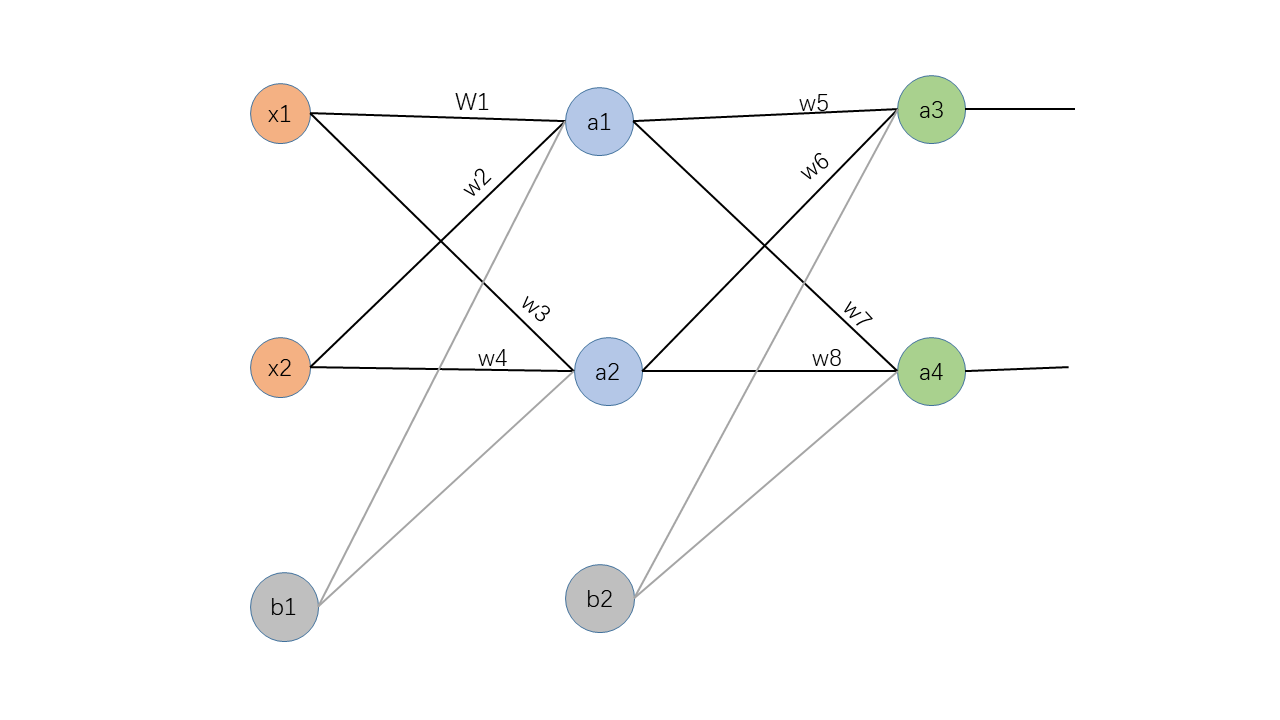
\includegraphics[scale=0.5]{bp2.png}
         \begin{flushleft}
            My derivation is about the picture above, and the following are the formulas I will use.$$Z = WA+b$$
            $$A = f(Z) = \frac{1}{1+e^{-Z}}$$
            $$L = \frac{1}{m}\sum_{i=1}^{m}(Y-A)^{2}$$  %均方误差
            The upper case letters in the formula are all matrix forms, I will first complete the computation one by one, and then simplify the expression in matrix form.
         \end{flushleft}
             
     \end{center}
     \subsection*{Forward propagation} 
     \begin{flushleft}
         
     \end{flushleft}

 \end{document}